\documentclass[sigconf, natbib=true]{acmart}
\usepackage{float}
\usepackage{booktabs} % For formal tables
\usepackage{url}
\usepackage{color}
\usepackage{enumitem}
\usepackage{multirow}
\usepackage{graphicx}
\usepackage{hyperref}
\hyphenation{Media-Eval}

% DOI
\acmDOI{}

% ISBN
\acmISBN{}

\settopmatter{printacmref=false}

\acmConference[DE'23-'24]{Data Engineering}{Radboud University}{Nijmegen, Netherlands} 
\acmYear{2024}
\copyrightyear{2024}

\setcopyright{none}

\graphicspath{{./images}}

\begin{document}
\title{Data Engineering --- Intermediate Report 4}

\author{Daan Brugmans (s1080742)}
\affiliation{%
    \institution{Radboud University} 
    \city{Nijmegen}
    \country{Netherlands}
}
\email{daan.brugmans@ru.nl}

\begin{abstract}
    This document is the final report for the Radboud University's Data Engineering course.
    Every section was written consecutively as a weekly assignment.
    The report describes the design and construction of a data pipeline.
    The code for the implementation of the pipeline described here can be found at the following URL: \url{https://github.com/daanbrugmans/ru-data-engineering-23-24}
\end{abstract}

\maketitle
% \begin{table}
%     \centering
%     \begin{tabular}{cols}
        
%     \end{tabular}
%     \caption{}
%     \label{tab:}
% \end{table}

% \begin{figure}
%     \centering
%     \includegraphics[width=0.9\textwidth]{}
%     \caption{}
%     \label{fig:}
% \end{figure}

\section{Data \& Project Proposal}
For the Data Engineering project, I would like to build a pipeline that serves data to data scientists working on a beer recommendation system.
The pipeline should collect from multiple sources that serve data(sets) of beer and their attributes.
Examples of attributes that should be served to the data scientists are name, brewery, alcohol by volume (ABV), international bitterness unit (IBU), category/style, textual description, flavor profile, personal ratings, and a timestamp.
The pipeline should serve two sets of data to the data scientists: a big general dataset containing beer data from varying publicly available sources that can (and should) be updated, and a small dataset of an end user of the beer recommendation system that includes personal ratings of beers the end user has had before.
These datasets will be served tabular.
The data scientists can then use the ratings of the end user and the data of both datasets to build a system that can recommend beers from the big dataset to the end user's non-specified preferences, which can be extracted from the end user's data using machine learning.
A realistic use case for such a recommendation system could exist for social media platforms revolving around beer and online retailers of beer that can use the system to increase revenue and beer sales.

% Maybe????
Due to the scope of the Data Engineering project, I will implement only the parts of the pipeline that are needed to serve the small dataset of an end user.
Although this requires that I construct a complete and working pipeline, I will move the focus away from data cleaning and joining, for example.

For the small dataset of an end user, I will provide my own data of beer ratings that I have collected on \citeauthor{untappd}.
\citet{untappd} is a social medium where users rate beers they try and share their ratings with friends by registering their rating on the medium ("check-in").
I participate in \citeauthor{untappd} and have collected a dataset of these check-ins with ratings.
I have access to an export of my check-in data via a GDPR request.
This export contains information about a beer's name, category/style, brewery, check-in location, purchasing location, flavor profile experienced by the end user, rating, and timestamp.
The data will be provided in CSV format and contain almost 400 check-ins, slightly over 300 of which being unique, so while I do not expect for missing data to be a major issue, duplicates will be more prominent.

% For the big dataset containing beers that can be recommended to an end user, I have found multiple data sources of beer attributes.
% I want to aggregate the data from these sources into a single database of beers. 
% Because my data sources serve data in varying formats, I expect that the aggregating of my data into a single collection will be a major challenge of the project.
% For example, I will have to make sure that all data uses the same formats and standards, that there are no duplicates due to beers being present in multiple sources, and that there will likely be missing data due to some data sources not storing certain attributes.

% I want to make use of the following data sources:
% \begin{itemize}
%     \item \citet{openbeerdb} is an archive of beer data.
%     Although it currently serves an older, static dataset, \citeauthor{openbeerdb} is planning on updating this dataset in the future, possibly including regular updates to the data.
%     The \citeauthor{openbeerdb} data is served as a set of \texttt{.sql} files that will create tables for beer, breweries, categories, and styles (finer granularity categories), and insert them with data.
%     The resulting SQL database contains most attributes I would want to serve to the data scientists, with the exception of flavor profile.
%     \item \citet{philipperemy} serves a static collection of beer data scraped from \citet{brewerydb}.
%     The dataset contains over 30,000 beers stored as JSON files, where every JSON file is a collection of beers.
%     The records contain almost all the data that I need, plus a lot more that I do not need, and seem quite complete.
%     The dataset size is ~80MBs.
    % \item \citet{evanhallmark} provides a dataset of beers, breweries, and beer reviews on Kaggle.
    % However, from Kaggle's preview, I have already noticed it contains several data quality issues: no documentation, missing data, strings that represent missing data, and the file for the reviews is over 2GBs.
    % The dataset consists of three CSV files, and the CSV for beer records contains almost 300,000 unique names.
% \end{itemize}

\section{Data Quality}
Before wrangling the data, I will talk about the data quality of the various data sources.
Quantitative measures of data quality were measured using code.
A class called the \texttt{DataQualityAssessor} assesses the data's quality using a few metrics.
A code snippet of this class can be found in figure \ref{fig:code_data_quality_assessor}.
This class is used in a Jupyter notebook that allows easy visualizations of data distributions and qualities.
This notebook can be found at the following URL: \url{https://github.com/daanbrugmans/ru-data-engineering-23-24/blob/main/code/analysis.ipynb}

\subsection{Untappd}
The Untappd data contains all of the features I need.
Most of these features do not have missing data: beer name, brewery name, beer type, ABV, IBU, personal rating, and check-in timestamp have 0\% data missing.

The flavor profiles experienced by the user have 1\% missing data, but since that's so little, I expect to be able to handle that issue easily.
The missing flavor profile data may be caused due to how a user selects flavors: although a user can select any combination of flavors from a set list, most users will often only select from the top 5 most chosen flavors for a beer, since \citeauthor{untappd} suggests those automatically.
Flavors that are not in the top 5 require more user interaction, and many users will refrain from manually searching for specific flavors.
This may mean that some beers with missing flavor profile data do have certain flavors as experienced by the user, but none of which being in the top 5 most chosen flavors, and the user did not manually search for the less common flavors.

More problematic is the feature for textual descriptions: 77\% of the check-ins do not have a textual comment, and of the remaining 23\%, not all comments are semantically relevant to the beer itself.
I expect that this feature is not one I can make good use of from the side of the personal dataset.
However, the general dataset will likely contain less missing descriptions, and the descriptions will likely be more factual and relevant to the beer itself.
The data scientists may use the textual descriptions from the general dataset for check-ins in the personalized dataset.

Based on box-and-whiskers-plot and barplot visualizations, there seem to be no outliers present in the data.
Two features are units of measure, ABV and IBU, and they are formatted correctly: ABV as a percentage, and IBU as a float.
The check-in timestamp is formatted to the standard ISO format, and floats use periods as the decimal mark.
The dataset is in an unnormalized form.

Although the Untappd data provides a unique ID for each record, for our purposes, that is not the primary key of our data: that would be beer name + brewery name.
We will assume that a brewery does not make multiple different beers that share the same name.
Given this primary key, the Untappd dataset consists of 18\% duplicates.
This can be fixed during data wrangling: duplicates are different check-ins of the same beer.
Features like beer name and brewery will be consistent across duplicates.
For some features, we must apply some transformation. 
For example, personal ratings can be averaged, and flavor profiles of all check-ins can be merged into one list.

% \subsection{OpenBeerDB}

% \subsection{BreweryDB}

\section{Data Wrangling}
Preferably, our pipeline should serve two different sets of data: the small personal dataset with a user's ratings, and the big general dataset to query beers from.
We will store these datasets as parquet files.
These datasets should share the same features, with the exception of the personal rating and the check-in timestamp for the personal dataset.
This list of features should be as follows:
\begin{itemize}
    \item Beer Name
    \item Brewery Name
    \item Beer Category (General)
    \item Beer Type (Specific)
    \item Alcohol By Volume (ABV)
    \item International Bitterness Unit (IBU)
    \item Textual Description
    \item Flavor Profile
\end{itemize}
We want to represent these features in a tabular manner.
Most of these features already fit this structure.
However, flavor profiles pose a problem, as they are currently stored as a list of varying size for every record in the \citeauthor{untappd} dataset.
My proposed solution is to wrangle the flavors into binary features: every flavor found in any flavor profile becomes a feature.
If a beer's flavor profile contains that flavor, the feature's value is 1, otherwise it is 0.
The main problem with this approach is that these flavor features are only stored in the \citeauthor{untappd} data.
If we want to use the features for the general dataset, we will have to extract that knowledge somehow.
For example, it could be collected from the \citeauthor{untappd} website, or the data scientists could use NLP techniques on a beer's name and description to fill in the features.
Regardless, making full use of the flavor features will require additional work.

The \citeauthor{untappd} dataset only has one column about beer category, but it actually contains both beer category and beer type: beer type is the full value, while beer category is the substring prior to the "-" (if it is present).

The \citeauthor{untappd} data source is currently represented in a tabular form and is stored in a CSV file.
I will wrangle it into the desired representation using Python and Pandas, applying further operations on dataframes.
Since all data is stored in a single CSV of manageable size, I can perform this process in bulk.
% All data sources are currently represented in a tabular form (\citeauthor{untappd}, \citeauthor{openbeerdb}) or a semi-structured form (\citeauthor{philipperemy}).
% The semi-structured data is represented using multiple JSON files of the same shape.
% I will wrangle it into a tabular format using Python and Pandas, applying further operations on dataframes.
% Since \citeauthor{openbeerdb}'s data is served as a set of SQL files that create tables with records to query, I will use SQL to get the features that I need, and wrangle those features using Python.
% I can perform this process in bulk.

% I want to join the datasets by \citet{openbeerdb} and \citet{philipperemy}, assuming a primary key of Beer Name + Brewery Name.
% However, this is not possible, because \citeauthor{philipperemy}'s dataset does not contain information about a beer's brewery.
% Although it would be possible to create a program that would try to scrape brewery information from \citeauthor{untappd}, for now, I will refrain from building such a program due to project scope constraints.
% Such a scraper could be worth the effort, though, since I could use it to fill in missing data, and standardize existing data to \citeauthor{untappd}'s standards.
% For now, my approach in joining this data shall be that I remove records from \citeauthor{philipperemy} with duplicate names, then join on Beer Name.

% Once the data for the general dataset has been joined, I will have to apply additional operations, because the different data sources have different possible sets of values for the same feature.
% The \citeauthor{untappd} dataset only has one column about beer category, but it actually contains both beer category and beer type: beer type is the full value, while beer category is the substring prior to the "-" (if it is present).
% The other datasets already have two different features for beer category and type, but sometimes use different names for the same category/type.
% Changing these values to be the same as the one in the personal dataset would improve data quality.

\section{Data Serving}
Serving of the data should be kept simple and designed to fit the stakeholders' needs.
Since these stakeholders are data scientists that want to have full access to all data, and since the data should not be accessible to the public, an API does not seem to be a good fit.
Currently, there is also no business logic that should be implemented, and the dataset size is small-scale and very manageable, so a QL API seems like an overengineered design for the current use case.
Since the data is personalized in nature, we should serve it with precautions and with as little data that could trace back to a person's identity.

A single parquet file should fit the data scientists' needs and would be preferred over CSV, but if the data scientists cannot perform their work with a parquet file, the data can be served as a CSV instead.
Assuming that the business can and is willing to cover the costs, serving the data using AWS S3 would be preferred over self-hosted alternatives, for the sake of the data lifecycle and infrastructure management.

Currently, the only data served is a small bulk file of the personal end user data of a single \citeauthor{untappd} user, which fits the serving design described above.
However, in the future, there may be many users whose check-ins we want to analyze.
If this number grows to be very big, we may want to partition the personal user data.
I propose that this partitioning is performed by a user's region/country.
This is because where a user lives has a major impact on what beers they may have access to; recommending local beers from the USA generally does not fit the needs of a German.
We should then also perform partitioning by region/country for the big general dataset, which is more likely to grow to a size too large for a single partition.
By using this partitioning scheme, we can recommend beers from the regions where people live, which makes it more likely that they can act upon (purchase) the recommendations.

If the size of the collected data is approaching a level where simply loading a single parquet file is not feasible anymore, only then should we consider implementing an API.
Such an API can map onto the partitions, serving a partition of the data for the region/country specified.

\section{Data Lifecycle}
It is expected that the pipeline described above will face challenges regarding the data lifecycle.
For example, we must anticipate that the general dataset is bound to grow.
Breweries will continue to make new beers on a regular basis, and these should be added to the general dataset.
Preferably, we try to synchronize the rate at which we update the general dataset with the pace at which breweries release new beers.
This could, for example, be weekly, fortnightly, or monthly, but should be based on general brewery release schedules.
By frequently adding to the general dataset, we can make sure that the end users of the beer recommendation system are able to purchase products that fit the current offerings.

Additionally, we should also frequently remove beers from the general dataset, since some beers have a limited production time, and it is useless to recommend beers to users when they cannot purchase them.
These deletions can occur less frequently than the additions, since beers going out of production is a less occurring phenomenon than new beers going into production.
For example, we could try a monthly or seasonal data destruction strategy.
This also goes for breweries, as sometimes, entire breweries go out of business.
When destroying beer data, we should also destroy data for all beers produced by a brewery that cannot offer them anymore.
Aside from these reasons for data destruction, we can assume that data in the general dataset will remain relevant indefinitely.
This is because most breweries have a core offering of products that they will always continue to produce.

The personal dataset of user check-ins and ratings has a higher need for being updated in a shorter time span than the general dataset.
This is because this data changes more frequently: an end user's list of checked-in beers can update weekly or even (nearly) daily, and we want to use that data for their recommendations.
We should attempt to also match this pace, updating end user data weekly or even daily in smaller batches.
This includes updating the ratings of existing check-ins if changed and deleting check-ins if a users chooses to, since the removal of check-ins reflects the apparent preferences of the end user.
We should also make sure that we can delete all check-ins of a user for GDPR compliance, but when using a pseudonymized ID for end user data, this should not be very difficult.

Furthermore, the timestamp of a user check-in should be considered.
This is because we may assume that more recent check-ins weigh more heavily than old check-ins, as a user's preferred tastes change over time.
We may still want to consider old check-ins nonetheless, so while we may not want to destroy old check-in data, it would be important for the data scientists to incorporate the time passed since a check-in into the recommendation system.

Given this information on the type and frequency of updates, I expect that a $\lambda$-Architecture would fit the pipeline best.
We want to update the data fairly frequently, but there is no need to do it very frequently (microbatching) or continuously (streaming).
I also expect that a row layout fits the data better than a columnar layout, since our updates will almost exclusively consist of data changes, and not schema changes.
We only expect to add new columns when a newly added beer contains a flavor in its flavor profile that does not exist in our dataset already.
We then have to add the flavor column to both datasets and set the newly added beer's value for that flavor to true and all other beers' value for that flavor to false.
Unfortunately, especially as the size of our data grows, this will be an expensive operation to make.
A potential solution would be to use \citeauthor{untappd}'s existing exhaustive list of flavors and adding all of these in advance.
Then, we would never have to apply schema changes, unless our data need changes.

Since we are serving parquet files, we can opt for a "Parquet S3 Zoo" strategy, where we host parquet files on AWS S3 that contain the data, and we keep adding new parquet files to S3 that contain information on how the existing parquet data has been deleted or updated.
We can use the DeltaLake or Iceberg framework as a tool to assist us in this in this strategy.

\bibliographystyle{ACM-Reference-Format}
\def\bibfont{\small} % comment this line for a smaller fontsize
\bibliography{refs.bib} 

\onecolumn
\appendix
\section{Appendix: Code Snippets}

\begin{figure*}[h]
    \centering
    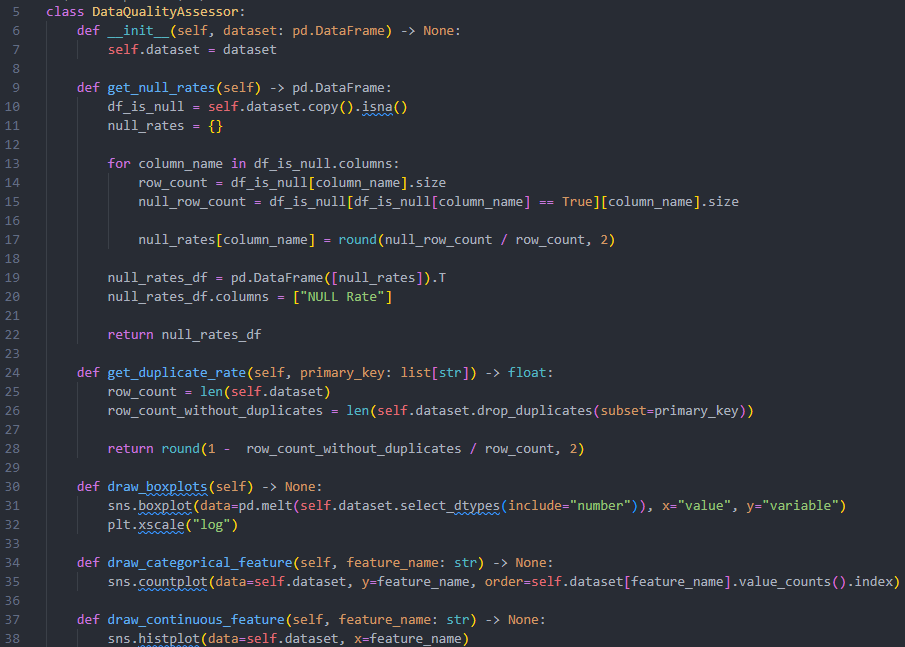
\includegraphics[width=0.9\textwidth]{code_data_quality_assessor.png}
    \caption{A code snippet for the \href{https://github.com/daanbrugmans/ru-data-engineering-23-24/blob/main/code/data_quality/data_quality_assessor.py}{Data Quality Assessor}.}
    \label{fig:code_data_quality_assessor}
\end{figure*}

\end{document}
